% Options for packages loaded elsewhere
\PassOptionsToPackage{unicode}{hyperref}
\PassOptionsToPackage{hyphens}{url}
\PassOptionsToPackage{dvipsnames,svgnames,x11names}{xcolor}
%
\documentclass[
  letterpaper,
  DIV=11,
  numbers=noendperiod]{scrreprt}

\usepackage{amsmath,amssymb}
\usepackage{lmodern}
\usepackage{iftex}
\ifPDFTeX
  \usepackage[T1]{fontenc}
  \usepackage[utf8]{inputenc}
  \usepackage{textcomp} % provide euro and other symbols
\else % if luatex or xetex
  \usepackage{unicode-math}
  \defaultfontfeatures{Scale=MatchLowercase}
  \defaultfontfeatures[\rmfamily]{Ligatures=TeX,Scale=1}
\fi
% Use upquote if available, for straight quotes in verbatim environments
\IfFileExists{upquote.sty}{\usepackage{upquote}}{}
\IfFileExists{microtype.sty}{% use microtype if available
  \usepackage[]{microtype}
  \UseMicrotypeSet[protrusion]{basicmath} % disable protrusion for tt fonts
}{}
\makeatletter
\@ifundefined{KOMAClassName}{% if non-KOMA class
  \IfFileExists{parskip.sty}{%
    \usepackage{parskip}
  }{% else
    \setlength{\parindent}{0pt}
    \setlength{\parskip}{6pt plus 2pt minus 1pt}}
}{% if KOMA class
  \KOMAoptions{parskip=half}}
\makeatother
\usepackage{xcolor}
\usepackage[normalem]{ulem}
\setlength{\emergencystretch}{3em} % prevent overfull lines
\setcounter{secnumdepth}{5}
% Make \paragraph and \subparagraph free-standing
\ifx\paragraph\undefined\else
  \let\oldparagraph\paragraph
  \renewcommand{\paragraph}[1]{\oldparagraph{#1}\mbox{}}
\fi
\ifx\subparagraph\undefined\else
  \let\oldsubparagraph\subparagraph
  \renewcommand{\subparagraph}[1]{\oldsubparagraph{#1}\mbox{}}
\fi

\usepackage{color}
\usepackage{fancyvrb}
\newcommand{\VerbBar}{|}
\newcommand{\VERB}{\Verb[commandchars=\\\{\}]}
\DefineVerbatimEnvironment{Highlighting}{Verbatim}{commandchars=\\\{\}}
% Add ',fontsize=\small' for more characters per line
\usepackage{framed}
\definecolor{shadecolor}{RGB}{241,243,245}
\newenvironment{Shaded}{\begin{snugshade}}{\end{snugshade}}
\newcommand{\AlertTok}[1]{\textcolor[rgb]{0.68,0.00,0.00}{#1}}
\newcommand{\AnnotationTok}[1]{\textcolor[rgb]{0.37,0.37,0.37}{#1}}
\newcommand{\AttributeTok}[1]{\textcolor[rgb]{0.40,0.45,0.13}{#1}}
\newcommand{\BaseNTok}[1]{\textcolor[rgb]{0.68,0.00,0.00}{#1}}
\newcommand{\BuiltInTok}[1]{\textcolor[rgb]{0.00,0.23,0.31}{#1}}
\newcommand{\CharTok}[1]{\textcolor[rgb]{0.13,0.47,0.30}{#1}}
\newcommand{\CommentTok}[1]{\textcolor[rgb]{0.37,0.37,0.37}{#1}}
\newcommand{\CommentVarTok}[1]{\textcolor[rgb]{0.37,0.37,0.37}{\textit{#1}}}
\newcommand{\ConstantTok}[1]{\textcolor[rgb]{0.56,0.35,0.01}{#1}}
\newcommand{\ControlFlowTok}[1]{\textcolor[rgb]{0.00,0.23,0.31}{#1}}
\newcommand{\DataTypeTok}[1]{\textcolor[rgb]{0.68,0.00,0.00}{#1}}
\newcommand{\DecValTok}[1]{\textcolor[rgb]{0.68,0.00,0.00}{#1}}
\newcommand{\DocumentationTok}[1]{\textcolor[rgb]{0.37,0.37,0.37}{\textit{#1}}}
\newcommand{\ErrorTok}[1]{\textcolor[rgb]{0.68,0.00,0.00}{#1}}
\newcommand{\ExtensionTok}[1]{\textcolor[rgb]{0.00,0.23,0.31}{#1}}
\newcommand{\FloatTok}[1]{\textcolor[rgb]{0.68,0.00,0.00}{#1}}
\newcommand{\FunctionTok}[1]{\textcolor[rgb]{0.28,0.35,0.67}{#1}}
\newcommand{\ImportTok}[1]{\textcolor[rgb]{0.00,0.46,0.62}{#1}}
\newcommand{\InformationTok}[1]{\textcolor[rgb]{0.37,0.37,0.37}{#1}}
\newcommand{\KeywordTok}[1]{\textcolor[rgb]{0.00,0.23,0.31}{#1}}
\newcommand{\NormalTok}[1]{\textcolor[rgb]{0.00,0.23,0.31}{#1}}
\newcommand{\OperatorTok}[1]{\textcolor[rgb]{0.37,0.37,0.37}{#1}}
\newcommand{\OtherTok}[1]{\textcolor[rgb]{0.00,0.23,0.31}{#1}}
\newcommand{\PreprocessorTok}[1]{\textcolor[rgb]{0.68,0.00,0.00}{#1}}
\newcommand{\RegionMarkerTok}[1]{\textcolor[rgb]{0.00,0.23,0.31}{#1}}
\newcommand{\SpecialCharTok}[1]{\textcolor[rgb]{0.37,0.37,0.37}{#1}}
\newcommand{\SpecialStringTok}[1]{\textcolor[rgb]{0.13,0.47,0.30}{#1}}
\newcommand{\StringTok}[1]{\textcolor[rgb]{0.13,0.47,0.30}{#1}}
\newcommand{\VariableTok}[1]{\textcolor[rgb]{0.07,0.07,0.07}{#1}}
\newcommand{\VerbatimStringTok}[1]{\textcolor[rgb]{0.13,0.47,0.30}{#1}}
\newcommand{\WarningTok}[1]{\textcolor[rgb]{0.37,0.37,0.37}{\textit{#1}}}

\providecommand{\tightlist}{%
  \setlength{\itemsep}{0pt}\setlength{\parskip}{0pt}}\usepackage{longtable,booktabs,array}
\usepackage{calc} % for calculating minipage widths
% Correct order of tables after \paragraph or \subparagraph
\usepackage{etoolbox}
\makeatletter
\patchcmd\longtable{\par}{\if@noskipsec\mbox{}\fi\par}{}{}
\makeatother
% Allow footnotes in longtable head/foot
\IfFileExists{footnotehyper.sty}{\usepackage{footnotehyper}}{\usepackage{footnote}}
\makesavenoteenv{longtable}
\usepackage{graphicx}
\makeatletter
\def\maxwidth{\ifdim\Gin@nat@width>\linewidth\linewidth\else\Gin@nat@width\fi}
\def\maxheight{\ifdim\Gin@nat@height>\textheight\textheight\else\Gin@nat@height\fi}
\makeatother
% Scale images if necessary, so that they will not overflow the page
% margins by default, and it is still possible to overwrite the defaults
% using explicit options in \includegraphics[width, height, ...]{}
\setkeys{Gin}{width=\maxwidth,height=\maxheight,keepaspectratio}
% Set default figure placement to htbp
\makeatletter
\def\fps@figure{htbp}
\makeatother

\KOMAoption{captions}{tableheading}
\makeatletter
\@ifpackageloaded{tcolorbox}{}{\usepackage[many]{tcolorbox}}
\@ifpackageloaded{fontawesome5}{}{\usepackage{fontawesome5}}
\definecolor{quarto-callout-color}{HTML}{909090}
\definecolor{quarto-callout-note-color}{HTML}{0758E5}
\definecolor{quarto-callout-important-color}{HTML}{CC1914}
\definecolor{quarto-callout-warning-color}{HTML}{EB9113}
\definecolor{quarto-callout-tip-color}{HTML}{00A047}
\definecolor{quarto-callout-caution-color}{HTML}{FC5300}
\definecolor{quarto-callout-color-frame}{HTML}{acacac}
\definecolor{quarto-callout-note-color-frame}{HTML}{4582ec}
\definecolor{quarto-callout-important-color-frame}{HTML}{d9534f}
\definecolor{quarto-callout-warning-color-frame}{HTML}{f0ad4e}
\definecolor{quarto-callout-tip-color-frame}{HTML}{02b875}
\definecolor{quarto-callout-caution-color-frame}{HTML}{fd7e14}
\makeatother
\makeatletter
\makeatother
\makeatletter
\@ifpackageloaded{caption}{}{\usepackage{caption}}
\AtBeginDocument{%
\ifdefined\contentsname
  \renewcommand*\contentsname{Table of contents}
\else
  \newcommand\contentsname{Table of contents}
\fi
\ifdefined\listfigurename
  \renewcommand*\listfigurename{List of Figures}
\else
  \newcommand\listfigurename{List of Figures}
\fi
\ifdefined\listtablename
  \renewcommand*\listtablename{List of Tables}
\else
  \newcommand\listtablename{List of Tables}
\fi
\ifdefined\figurename
  \renewcommand*\figurename{Figure}
\else
  \newcommand\figurename{Figure}
\fi
\ifdefined\tablename
  \renewcommand*\tablename{Table}
\else
  \newcommand\tablename{Table}
\fi
}
\@ifpackageloaded{float}{}{\usepackage{float}}
\floatstyle{ruled}
\@ifundefined{c@chapter}{\newfloat{codelisting}{h}{lop}}{\newfloat{codelisting}{h}{lop}[chapter]}
\floatname{codelisting}{Listing}
\newcommand*\listoflistings{\listof{codelisting}{List of Listings}}
\makeatother
\makeatletter
\@ifpackageloaded{caption}{}{\usepackage{caption}}
\@ifpackageloaded{subcaption}{}{\usepackage{subcaption}}
\makeatother
\makeatletter
\@ifpackageloaded{tcolorbox}{}{\usepackage[many]{tcolorbox}}
\makeatother
\makeatletter
\@ifundefined{shadecolor}{\definecolor{shadecolor}{rgb}{.97, .97, .97}}
\makeatother
\makeatletter
\makeatother
\ifLuaTeX
  \usepackage{selnolig}  % disable illegal ligatures
\fi
\IfFileExists{bookmark.sty}{\usepackage{bookmark}}{\usepackage{hyperref}}
\IfFileExists{xurl.sty}{\usepackage{xurl}}{} % add URL line breaks if available
\urlstyle{same} % disable monospaced font for URLs
\hypersetup{
  pdftitle={Casual Musings on   Data Structures and Algorithms},
  pdfauthor={Neeldhara Misra},
  colorlinks=true,
  linkcolor={blue},
  filecolor={Maroon},
  citecolor={Blue},
  urlcolor={Blue},
  pdfcreator={LaTeX via pandoc}}

\title{Casual Musings on Data Structures and Algorithms}
\author{Neeldhara Misra}
\date{8/2/2022}

\begin{document}
\maketitle
\ifdefined\Shaded\renewenvironment{Shaded}{\begin{tcolorbox}[interior hidden, breakable, enhanced, boxrule=0pt, frame hidden, sharp corners, borderline west={3pt}{0pt}{shadecolor}]}{\end{tcolorbox}}\fi

\renewcommand*\contentsname{Table of contents}
{
\hypersetup{linkcolor=}
\setcounter{tocdepth}{2}
\tableofcontents
}
\hypertarget{preface}{%
\chapter*{Preface}\label{preface}}
\addcontentsline{toc}{chapter}{Preface}

\begin{center}\rule{0.5\linewidth}{0.5pt}\end{center}

These are running notes from my course on Data Structures and Algorithms
at IIT Gandhinagar.

If you would like to have access to the weekly assignments, you might
want to \href{https://neeldhara.courses/}{register for the course here}
(it's free).

If you have any general comments or questions, please leave them below.
Thanks!

\hypertarget{hyvor-talk-view}{}

\hypertarget{data-structures-and-structured-data}{%
\chapter{Data Structures and Structured
Data}\label{data-structures-and-structured-data}}

\href{https://slides.com/neeldhara/dsa1-w01}{Link to Slides}

\hypertarget{wdym-data-structures}{%
\section{WDYM, data structures?}\label{wdym-data-structures}}

We will keep it casual and skip formal definitions for now. 👀

Data structures give us principled ways to \emph{stow away} information.
It's important to do this nicely based on what you want to \emph{do}
with the information.

For example, the notes you might be taking in this class is information.
If you have no plans of revisiting them later, you can take them as you
please, or better yet, not take them at all!

However, you want your notes optimised for giving you quality company
during a 2AM revision session on exam day, competing with Maggi for
attention, you want your notes to be competently taken: they don't have
to be neat, and it's enough for them to be useful.

On the other hand, if you are taking notes so that a special someone who
will inevitably miss a few classes will almost certainly ask for later,
then you would be making notes to impress, and that potentially requires
a different approach.

\begin{tcolorbox}[standard jigsaw,toptitle=1mm, titlerule=0mm, bottomtitle=1mm, title=\textcolor{quarto-callout-tip-color}{\faLightbulb}\hspace{0.5em}{Throughout this course, we will try to make sense of trade-offs.}, coltitle=black, colback=white, toprule=.15mm, colframe=quarto-callout-tip-color-frame, arc=.35mm, rightrule=.15mm, opacityback=0, left=2mm, leftrule=.75mm, colbacktitle=quarto-callout-tip-color!10!white, opacitybacktitle=0.6, bottomrule=.15mm]
We'll equip ourselves with ideas that will ultimately help you decide
questions like: how do you organise the clothes in your cupboard?

\begin{longtable}[]{@{}
  >{\raggedright\arraybackslash}p{(\columnwidth - 4\tabcolsep) * \real{0.1975}}
  >{\raggedright\arraybackslash}p{(\columnwidth - 4\tabcolsep) * \real{0.3704}}
  >{\raggedright\arraybackslash}p{(\columnwidth - 4\tabcolsep) * \real{0.4321}}@{}}
\toprule()
\begin{minipage}[b]{\linewidth}\raggedright
\end{minipage} & \begin{minipage}[b]{\linewidth}\raggedright
Throw 'em in, nobody's looking
\end{minipage} & \begin{minipage}[b]{\linewidth}\raggedright
Keep it where you can find it later
\end{minipage} \\
\midrule()
\endhead
Time to process & Negligible & Forever \\
Time to retrieve & Forever & Negligible \\
\bottomrule()
\end{longtable}

Table 1. No free lunches.
\end{tcolorbox}

\begin{tcolorbox}[standard jigsaw,toptitle=1mm, titlerule=0mm, bottomtitle=1mm, title=\textcolor{quarto-callout-note-color}{\faInfo}\hspace{0.5em}{This \emph{is} in fact a useful framing!}, coltitle=black, colback=white, toprule=.15mm, colframe=quarto-callout-note-color-frame, arc=.35mm, rightrule=.15mm, opacityback=0, left=2mm, leftrule=.75mm, colbacktitle=quarto-callout-note-color!10!white, opacitybacktitle=0.6, bottomrule=.15mm]
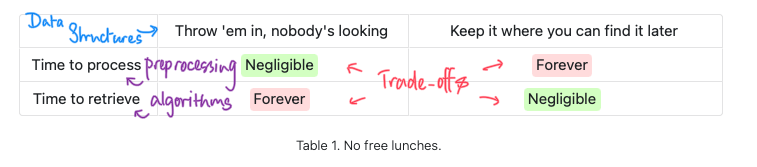
\includegraphics{./figures/ch1-table01.png}
\end{tcolorbox}

\hypertarget{representing-polynomials}{%
\section{Representing Polynomials}\label{representing-polynomials}}

Let's say that you are spending a fine evening watching the
\#LockdownMath playlist from 3blue1brown. The first episode happens to
be all about solving quadratics:

\begin{figure}

{\centering 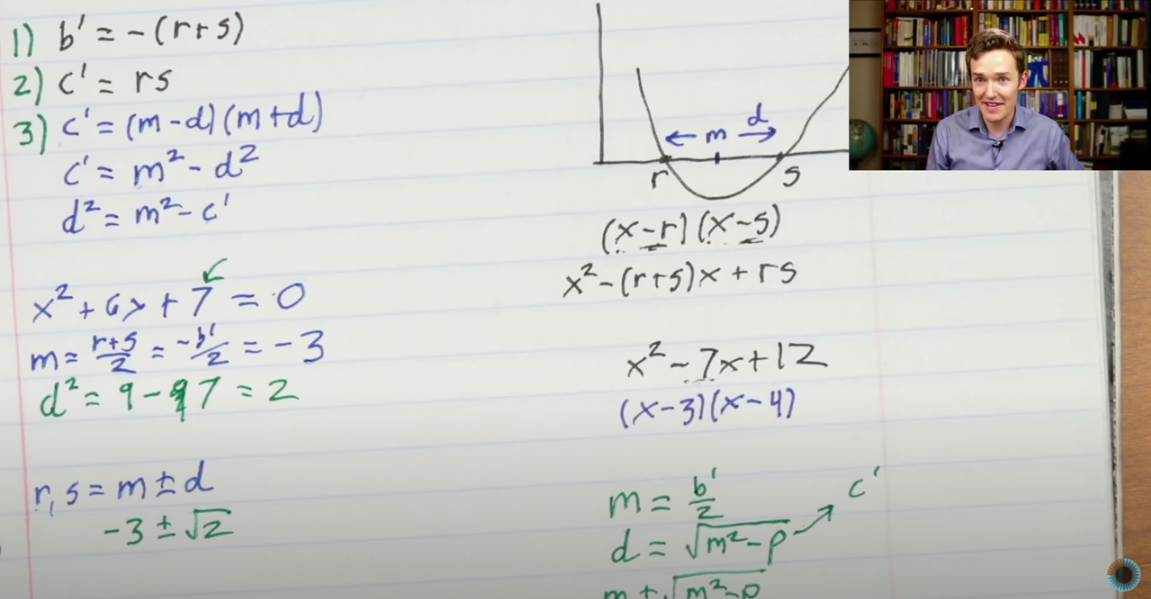
\includegraphics{./figures/ch1-lockdownmath.png}

}

\caption{A screenshot from \#LockdownMath showing Grant Sanderson
solving quadratics.}

\end{figure}

Now, it's quite natural to want to ``write a program'', so to speak,
that can take a quadratic equation such as \(x^2 - 7x + 12\) as input
and output its two roots.

Given that programs running on your phone are able to make suggestions,
even if dubious, for what series to binge-watch next on Netflix, finding
roots of quadratics should be a fairly benign exercise.

You might recall that most programs let you declare variables that can
hold on to specific \emph{types} of information, for instance: numbers,
strings, and so forth. Our input doesn't ``look'' like a number, so it
would be a fair take to simply store it as a string:

\begin{Shaded}
\begin{Highlighting}[]
\NormalTok{px }\OperatorTok{=} \StringTok{"x\^{}2 {-} 7x + 12"}\OperatorTok{;}
\end{Highlighting}
\end{Shaded}

\begin{tcolorbox}[standard jigsaw,toptitle=1mm, titlerule=0mm, bottomtitle=1mm, title=\textcolor{quarto-callout-note-color}{\faInfo}\hspace{0.5em}{Now\ldots{}}, coltitle=black, colback=white, toprule=.15mm, colframe=quarto-callout-note-color-frame, arc=.35mm, rightrule=.15mm, opacityback=0, left=2mm, leftrule=.75mm, colbacktitle=quarto-callout-note-color!10!white, opacitybacktitle=0.6, bottomrule=.15mm]

\includegraphics{./figures/ch1-meme01.jpeg}
\end{tcolorbox}

While this is a perfectly faithful representation, you can imagine that
it would be slightly painful to work with. You would have to write some
code that can ``pull out'' the parts of the string that represent the
\emph{numbers} you care about (in this example, \(b = -7\) and
\(c = 12\)), so that you can move on to your calculation, which is an
\emph{expression} involving numbers.

Given that a quadratic with the leading coefficient normalized to one is
uniquely determined by two numbers, it seems a lot simpler to directly
represent the polynomial as two integers instead:

\begin{Shaded}
\begin{Highlighting}[]
\NormalTok{px\_b }\OperatorTok{=} \OperatorTok{{-}}\DecValTok{7}
\NormalTok{px\_c }\OperatorTok{=} \DecValTok{12}
\end{Highlighting}
\end{Shaded}

You might appreciate that this saves us quite some circus and we can
quite directly get to the computation we're interested in. What if you
cared about higher order polynomials? You may want to solve them (even
if you
\href{https://www.youtube.com/watch?t=2543\&v=O5eH3x3sTNA\&feature=youtu.be}{run
out of expressions for solutions pretty quickly}, you might be
interested in \href{https://math.stackexchange.com/a/1386830}{other ways
of getting to the roots}), or manipulate them in other ways (for
example, by adding or
\href{https://www.youtube.com/watch?v=h7apO7q16V0}{multiplying} them).

\begin{tcolorbox}[standard jigsaw,toptitle=1mm, titlerule=0mm, bottomtitle=1mm, title=\textcolor{quarto-callout-caution-color}{\faFire}\hspace{0.5em}{Food for thought.}, coltitle=black, colback=white, toprule=.15mm, colframe=quarto-callout-caution-color-frame, arc=.35mm, rightrule=.15mm, opacityback=0, left=2mm, leftrule=.75mm, colbacktitle=quarto-callout-caution-color!10!white, opacitybacktitle=0.6, bottomrule=.15mm]
How would you represent higher-order polynomials? What about
multivariate polynomials? Is there a way that you might be able to
capture an algebraic expression for a polynomial without either using
strings or just the coefficients?
\end{tcolorbox}

\hypertarget{representing-a-game---i}{%
\section{Representing a Game - I}\label{representing-a-game---i}}

The \href{https://www.youtube.com/watch?v=846A4rgO_os}{game of 100} goes
like this: I pick a number between 1 and 10, and then you pick one
within the next ten numbers, and on and on. The first person to reach
100 wins.

\begin{tcolorbox}[standard jigsaw,toptitle=1mm, titlerule=0mm, bottomtitle=1mm, title=\textcolor{quarto-callout-note-color}{\faInfo}\hspace{0.5em}{Recall from class and/or figure out that\ldots{}}, coltitle=black, colback=white, toprule=.15mm, colframe=quarto-callout-note-color-frame, arc=.35mm, rightrule=.15mm, opacityback=0, left=2mm, leftrule=.75mm, colbacktitle=quarto-callout-note-color!10!white, opacitybacktitle=0.6, bottomrule=.15mm]

\begin{tcolorbox}[standard jigsaw,toptitle=1mm, titlerule=0mm, bottomtitle=1mm, title=\textcolor{quarto-callout-warning-color}{\faExclamationTriangle}\hspace{0.5em}{SPOILER ALERT}, coltitle=black, colback=white, toprule=.15mm, colframe=quarto-callout-warning-color-frame, arc=.35mm, rightrule=.15mm, opacityback=0, left=2mm, leftrule=.75mm, colbacktitle=quarto-callout-warning-color!10!white, opacitybacktitle=0.6, bottomrule=.15mm]

\begin{verbatim}
...whoever starts has a way of winning the game:

    0. To begin with, I say 1. 
    1. No matter what number you pick, I can say 12.
    2. No matter what number you pick, I can say 23.
    3. No matter what number you pick, I can say 34.
    4. No matter what number you pick, I can say 45.
    5. No matter what number you pick, I can say 56.
    6. No matter what number you pick, I can say 67.
    7. No matter what number you pick, I can say 78.
    8. No matter what number you pick, I can say 89.
    9. No matter what number you pick, I can say 100.
\end{verbatim}

\end{tcolorbox}

\end{tcolorbox}

What if you want to write a program that mimics the winning strategy?

Note that this game can go on for at most a 100 steps, and in fact
exactly 20 steps (or ten rounds) when you employ said winning strategy.
So one way to go about this is to declare 20 variables to track the 20
numbers exchanged between the players. But a moment's reflection may
reveal that you \emph{don't} need to store anything at all.

\begin{tcolorbox}[standard jigsaw,toptitle=1mm, titlerule=0mm, bottomtitle=1mm, title=\textcolor{quarto-callout-caution-color}{\faFire}\hspace{0.5em}{Exercise}, coltitle=black, colback=white, toprule=.15mm, colframe=quarto-callout-caution-color-frame, arc=.35mm, rightrule=.15mm, opacityback=0, left=2mm, leftrule=.75mm, colbacktitle=quarto-callout-caution-color!10!white, opacitybacktitle=0.6, bottomrule=.15mm]
Can you write a program that makes the first move, prompts the user for
their moves on their turn, uses the winning strategy discussed above,
and uses no variables for explicit storage?
\end{tcolorbox}

\hypertarget{representing-a-game---ii}{%
\section{Representing a Game - II}\label{representing-a-game---ii}}

If \sout{you missed the first class} you haven't played the
\href{https://ncase.me/trust/}{Game of Trust}, you are welcome to take a
break and experience it now. Let's recollect the setup:

\begin{figure}

{\centering 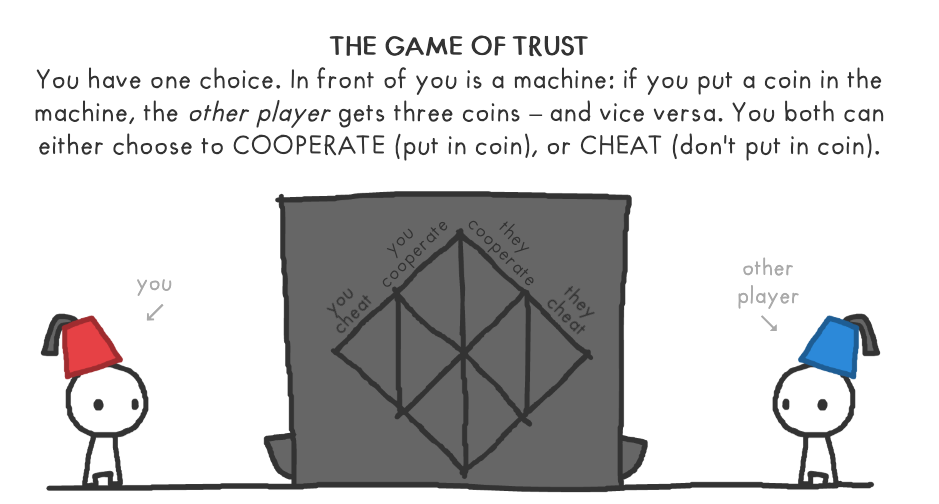
\includegraphics{./figures/ch1-game-trust.png}

}

\caption{Illustration from an implementation by
\href{https://ncase.me/trust/}{Nicky Case}.}

\end{figure}

Suppose you want to implement your own version of this game, where the
program responds to inputs from the user and plays according to a
specific, pre-meditated strategy. Remember you have seen some strategies
already:

\begin{figure}

{\centering 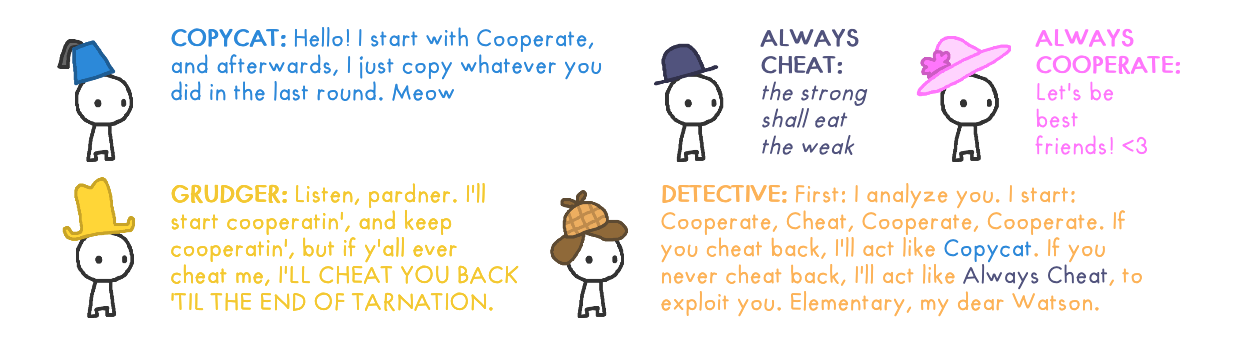
\includegraphics{./figures/ch1-players-trust.png}

}

\caption{A second illustration from the same implementation by
\href{https://ncase.me/trust/}{Nicky Case}.}

\end{figure}

We reproduce these strategies below:

\begin{tcolorbox}[standard jigsaw,toptitle=1mm, titlerule=0mm, bottomtitle=1mm, title=\textcolor{quarto-callout-note-color}{\faInfo}\hspace{0.5em}{Player Strategies}, coltitle=black, colback=white, toprule=.15mm, colframe=quarto-callout-note-color-frame, arc=.35mm, rightrule=.15mm, opacityback=0, left=2mm, leftrule=.75mm, colbacktitle=quarto-callout-note-color!10!white, opacitybacktitle=0.6, bottomrule=.15mm]

\begin{enumerate}
\def\labelenumi{\arabic{enumi}.}
\tightlist
\item
  COPYCAT: Hello! I start with Cooperate, and afterwards, I just copy
  whatever you did in the last round. Meow.
\item
  ALWAYS CHEAT: The strong shall eat the weak.
\item
  ALWAYS COOPERATE: Let's be best friends \textless3
\item
  GRUDGER: Listen, pardner. I'll start cooperatin', and keep
  cooperatin', but if y'all ever cheat me, I'LL CHEAT YOU BACK TIL THE
  END OF TARNATION.
\item
  DETECTIVE: First: I analyze you. start: Cooperate, Cheat, Cooperate,
  Cooperate. If you cheat back, I'll act like Copycat. If you never
  cheat back, I'll act like Always Cheat, to exploit you. Elementary, my
  dear Watson.
\end{enumerate}

\end{tcolorbox}

Let's say that your program is designed to play 5 rounds and that your
program is playing the copycat strategy. To begin with, you might want
to declare a couple of variables to keep track of the scores of the
players, and ten variables to track the moves of both players in each
round. With this, your code may start out looking like this:

\begin{Shaded}
\begin{Highlighting}[]
\NormalTok{my\_points }\OperatorTok{=} \DecValTok{0}
\NormalTok{user\_points }\OperatorTok{=} \DecValTok{0}

\NormalTok{user\_move\_1 }\OperatorTok{=} \FunctionTok{input}\OperatorTok{(}\StringTok{"Input 1 for Cooperate and 0 for Cheat."}\OperatorTok{)}

\CommentTok{//Sanity check input:}
\ControlFlowTok{if}\OperatorTok{(}\NormalTok{user\_move\_1 }\OperatorTok{!=} \DecValTok{1}\NormalTok{ and user\_move\_1 }\OperatorTok{!=} \DecValTok{0}\OperatorTok{):}
\NormalTok{    express disappointment and abort}
\end{Highlighting}
\end{Shaded}

\begin{Shaded}
\begin{Highlighting}[]
\CommentTok{// My first move is to cooperate:}
\NormalTok{my\_points }\OperatorTok{+=} \OperatorTok{{-}}\DecValTok{1}
\NormalTok{user\_points }\OperatorTok{+=} \DecValTok{3}

\ControlFlowTok{if}\OperatorTok{(}\NormalTok{user\_move\_1}\OperatorTok{):}
\NormalTok{    my\_points }\OperatorTok{+=} \DecValTok{3}
\NormalTok{    user\_points }\OperatorTok{{-}=} \DecValTok{1}
\end{Highlighting}
\end{Shaded}

Now your next move is determined by the value of \texttt{user\_move\_1},
so you might proceed as follows.

\begin{Shaded}
\begin{Highlighting}[]
\NormalTok{user\_move\_2 }\OperatorTok{=} \FunctionTok{input}\OperatorTok{(}\StringTok{"Input 1 for Cooperate and 0 for Cheat."}\OperatorTok{)}

\CommentTok{//Sanity check input:}
\ControlFlowTok{if}\OperatorTok{(}\NormalTok{user\_move\_2 }\OperatorTok{!=} \DecValTok{1}\NormalTok{ and user\_move\_2 }\OperatorTok{!=} \DecValTok{0}\OperatorTok{):}
\NormalTok{    express disappointment and abort}
\end{Highlighting}
\end{Shaded}

\begin{Shaded}
\begin{Highlighting}[]
\CommentTok{// My next move is based on the user\textquotesingle{}s first:}
\ControlFlowTok{if}\OperatorTok{(}\NormalTok{user\_move\_1}\OperatorTok{):}
\NormalTok{    my\_points }\OperatorTok{+=} \OperatorTok{{-}}\DecValTok{1}
\NormalTok{    user\_points }\OperatorTok{+=} \DecValTok{3}

\ControlFlowTok{if}\OperatorTok{(}\NormalTok{user\_move\_2}\OperatorTok{):}
\NormalTok{    my\_points }\OperatorTok{+=} \DecValTok{3}
\NormalTok{    user\_points }\OperatorTok{{-}=} \DecValTok{1}
\end{Highlighting}
\end{Shaded}

\ldots and so on and on, you get the drift.

\begin{tcolorbox}[standard jigsaw,toptitle=1mm, titlerule=0mm, bottomtitle=1mm, title=\textcolor{quarto-callout-caution-color}{\faFire}\hspace{0.5em}{Food for thought.}, coltitle=black, colback=white, toprule=.15mm, colframe=quarto-callout-caution-color-frame, arc=.35mm, rightrule=.15mm, opacityback=0, left=2mm, leftrule=.75mm, colbacktitle=quarto-callout-caution-color!10!white, opacitybacktitle=0.6, bottomrule=.15mm]
Do you really need ten variables to track the game? If you were instead
implementing the always cheat or always cooperate strategy, how many
variables would you need? What about the strategies of the grudger and
the detective?
\end{tcolorbox}

Now, suppose we come up with our own player, whom we call the
\textbf{majority mover}. This player looks at your entire game history,
and cooperates if you have cooperated more than you have cheated, and
cheats if you have cheated more than you have cooperated, and acts
randomly otherwise.

It seems like implementing the majority mover strategy would really
require keeping track of everything. Or would it? You might observe at
this point that it's enough to keep track of two counts: the number of
rounds and the \emph{number} of moves where the user has cheated: note
that it does not matter when the cheats happened in the history of the
game.

\begin{tcolorbox}[standard jigsaw,toptitle=1mm, titlerule=0mm, bottomtitle=1mm, title=\textcolor{quarto-callout-note-color}{\faInfo}\hspace{0.5em}{You could also\ldots{}}, coltitle=black, colback=white, toprule=.15mm, colframe=quarto-callout-note-color-frame, arc=.35mm, rightrule=.15mm, opacityback=0, left=2mm, leftrule=.75mm, colbacktitle=quarto-callout-note-color!10!white, opacitybacktitle=0.6, bottomrule=.15mm]
\ldots track the number of cooperate moves along with the number of
rounds; or the number of cheat moves and the number of cooperate moves.

At this point it's a matter of taste :)
\end{tcolorbox}

How about a \textbf{completely random} player? This one chooses a number
\textbf{K} between 1 and N uniformly at random (let's not worry about
\emph{how} this is done for now, because that would be a story for
another day), where N is the number of rounds played so far; and mimics
the other player's \textbf{K}th move. To implement this strategy, you
really would need to keep track of the user's entire game history with
the five variables, and also assume that you have a way of picking a
number at random.

Finally, consider that instead of fixing your program to play five
rounds --- 🥱 --- you want to politely ask the user how m\emph{any
}rounds they want to play.

\begin{tcolorbox}[standard jigsaw,toptitle=1mm, titlerule=0mm, bottomtitle=1mm, title=\textcolor{quarto-callout-note-color}{\faInfo}\hspace{0.5em}{After all\ldots{}}, coltitle=black, colback=white, toprule=.15mm, colframe=quarto-callout-note-color-frame, arc=.35mm, rightrule=.15mm, opacityback=0, left=2mm, leftrule=.75mm, colbacktitle=quarto-callout-note-color!10!white, opacitybacktitle=0.6, bottomrule=.15mm]

\includegraphics{./figures/ch1-meme02.jpeg}
\end{tcolorbox}

Well, for the first few players, this is just a matter of upgrading your
for loop (which you should have switched to already when you realised
that you don't need all. those. variables.) to use N: and you are done.

\begin{tcolorbox}[standard jigsaw,toptitle=1mm, titlerule=0mm, bottomtitle=1mm, title=\textcolor{quarto-callout-caution-color}{\faFire}\hspace{0.5em}{Food for thought.}, coltitle=black, colback=white, toprule=.15mm, colframe=quarto-callout-caution-color-frame, arc=.35mm, rightrule=.15mm, opacityback=0, left=2mm, leftrule=.75mm, colbacktitle=quarto-callout-caution-color!10!white, opacitybacktitle=0.6, bottomrule=.15mm]
How will you implement this version if you are working with our latest
player? If you happen to have a very enthusiastic user who asks for half
a million rounds, would you be able to declare that many variables all
at once, while your program is running? Notably, you don't know what the
user is going to say ahead of time!
\end{tcolorbox}

\hypertarget{representing-a-subset-of-a-deck-of-cards}{%
\section{Representing a subset of a deck of
cards}\label{representing-a-subset-of-a-deck-of-cards}}

If you are implementing a card\footnote{Assume you are working with the
  \href{https://en.wikipedia.org/wiki/Standard_52-card_deck}{standard
  52-card deck}.} game, you might need a mechanism for keeping track of
``hands'', or various subsets of cards. Let's say a \emph{hand} is a
subset of cards. For many games, you would need the ability to be able
to quickly:

\begin{itemize}
\tightlist
\item
  tell if a particular card belongs to a hand or not,
\item
  add a card to a hand,
\item
  remove a card from a hand, and
\item
  replace a card in a hand with another one.
\end{itemize}

One way to meet these requirements is to declare a collection of 52
boolean (i.e, true/false or 0/1) variables to represent the hand: the
cards in the hand are set to true while cards that don't belong are set
to false.

\begin{tcolorbox}[standard jigsaw,toptitle=1mm, titlerule=0mm, bottomtitle=1mm, title=\textcolor{quarto-callout-caution-color}{\faFire}\hspace{0.5em}{Food for thought.}, coltitle=black, colback=white, toprule=.15mm, colframe=quarto-callout-caution-color-frame, arc=.35mm, rightrule=.15mm, opacityback=0, left=2mm, leftrule=.75mm, colbacktitle=quarto-callout-caution-color!10!white, opacitybacktitle=0.6, bottomrule=.15mm]
What do you like about this method? What don't you like about it?
\end{tcolorbox}

Here'a another way, though: you could agree on a notation for the cards
in the deck: e.g, a standard one is to use a number, A/J/Q/K to denote
the value, and S/C/D/H to denote the suit, so every card can be
represented as a pair of characters. For example the Ace of Diamonds
would be AD, the five of spades would be 5S and the King of Hearts would
be KH. With this in place, you could represent a hand also by simply
\emph{concatenating} these string representations of the hards in the
hand.

\begin{tcolorbox}[standard jigsaw,toptitle=1mm, titlerule=0mm, bottomtitle=1mm, title=\textcolor{quarto-callout-caution-color}{\faFire}\hspace{0.5em}{Food for thought.}, coltitle=black, colback=white, toprule=.15mm, colframe=quarto-callout-caution-color-frame, arc=.35mm, rightrule=.15mm, opacityback=0, left=2mm, leftrule=.75mm, colbacktitle=quarto-callout-caution-color!10!white, opacitybacktitle=0.6, bottomrule=.15mm]
What do you like about this method? What don't you like about it?
\end{tcolorbox}

Now for this toy example, if you were to implement both methods and
clock the time taken to implement the four operations above, you may not
notice a major difference. However, for actual applications, you may be
in a situation where your \emph{subsets} (here, the ``hands'') may be
coming from a large \emph{universe} (here, the ``deck''). On the other
hand, you may have a very large number of operations to take care of
efficiently.

\begin{tcolorbox}[standard jigsaw,toptitle=1mm, titlerule=0mm, bottomtitle=1mm, title=\textcolor{quarto-callout-caution-color}{\faFire}\hspace{0.5em}{Food for thought.}, coltitle=black, colback=white, toprule=.15mm, colframe=quarto-callout-caution-color-frame, arc=.35mm, rightrule=.15mm, opacityback=0, left=2mm, leftrule=.75mm, colbacktitle=quarto-callout-caution-color!10!white, opacitybacktitle=0.6, bottomrule=.15mm]
Are there other ways that you might want to store this kind of
information, given the things you want to do are as enlisted above?
\end{tcolorbox}

Your choice of method will again be driven by the requirements: the one
thing to keep in mind is that you cannot have it all, but we can usually
get pretty damn close!

\begin{center}\rule{0.5\linewidth}{0.5pt}\end{center}

\hypertarget{hyvor-talk-view}{}

\hypertarget{playlists-and-tweet-threads-representing-sequential-information}{%
\chapter{\texorpdfstring{Playlists and Tweet Threads: Representing
Sequential
Information}{Playlists and Tweet Threads:  Representing Sequential Information}}\label{playlists-and-tweet-threads-representing-sequential-information}}

\href{hhttps://slides.com/neeldhara/dsa1-w01\#/2/1}{Link to Slides}

(Coming soon.)

\hypertarget{when-the-relationship-status-is-simple-representing-graphs.}{%
\chapter{\texorpdfstring{When the Relationship Status is Simple:
Representing
Graphs.}{When the Relationship Status is Simple:  Representing Graphs.}}\label{when-the-relationship-status-is-simple-representing-graphs.}}

\hypertarget{drawing-and-walking-challenges}{%
\section{Drawing and Walking
Challenges}\label{drawing-and-walking-challenges}}

At some point of time in your life, you have likely been challenged to
draw a kite-like figure:

\begin{figure}

{\centering 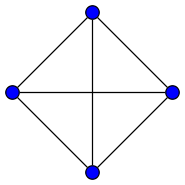
\includegraphics{./figures/draw-K4.png}

}

\caption{A common drawing challenge.}

\end{figure}

without ever lifting your pencil/pen/quill off the paper. You may have
noticed that there are figures that are particularly elusive to this
persistent style of drawing, while others are pleasingly possible to
draw in this fashion.

\begin{tcolorbox}[standard jigsaw,toptitle=1mm, titlerule=0mm, bottomtitle=1mm, title=\textcolor{quarto-callout-warning-color}{\faExclamationTriangle}\hspace{0.5em}{(Spoiler) Beth Thomas demonstrating what drawing challenges are doable}, coltitle=black, colback=white, toprule=.15mm, colframe=quarto-callout-warning-color-frame, arc=.35mm, rightrule=.15mm, opacityback=0, left=2mm, leftrule=.75mm, colbacktitle=quarto-callout-warning-color!10!white, opacitybacktitle=0.6, bottomrule=.15mm]

\end{tcolorbox}

The city of Königsberg in Prussia (now Kaliningrad, Russia) was set on
both sides of the Pregel River, and included two large
islands---Kneiphof and Lomse---which were connected to each other, and
to the two mainland portions of the city, by seven bridges.

\begin{tcolorbox}[standard jigsaw,toptitle=1mm, titlerule=0mm, bottomtitle=1mm, title=\textcolor{quarto-callout-caution-color}{\faFire}\hspace{0.5em}{The Problem}, coltitle=black, colback=white, toprule=.15mm, colframe=quarto-callout-caution-color-frame, arc=.35mm, rightrule=.15mm, opacityback=0, left=2mm, leftrule=.75mm, colbacktitle=quarto-callout-caution-color!10!white, opacitybacktitle=0.6, bottomrule=.15mm]
Devise a walk through the city that would cross each of those bridges
once and only once. Try this yourself on a few different maps at
\href{https://mathigon.org/course/graph-theory/bridges}{Mathigon}!
\end{tcolorbox}

\begin{figure}

{\centering 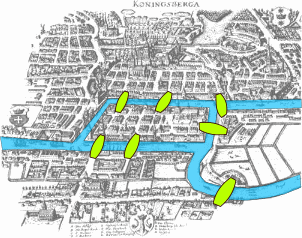
\includegraphics{./figures/ch3-knbridges.png}

}

\caption{Konigsberg Classic: Map of Königsberg in Euler's time showing
the actual layout of the seven bridges, highlighting the river Pregel
and the bridges. Image by Bogdan Giuşcă, in the public domain (CC BY-SA
3.0) and sourced from Wikipedia.}

\end{figure}

\begin{tcolorbox}[standard jigsaw,toptitle=1mm, titlerule=0mm, bottomtitle=1mm, title=\textcolor{quarto-callout-warning-color}{\faExclamationTriangle}\hspace{0.5em}{(Spoiler) Numberphile commentary on the bridges of Königsberg}, coltitle=black, colback=white, toprule=.15mm, colframe=quarto-callout-warning-color-frame, arc=.35mm, rightrule=.15mm, opacityback=0, left=2mm, leftrule=.75mm, colbacktitle=quarto-callout-warning-color!10!white, opacitybacktitle=0.6, bottomrule=.15mm]

\end{tcolorbox}

\begin{tcolorbox}[standard jigsaw,toptitle=1mm, titlerule=0mm, bottomtitle=1mm, title=\textcolor{quarto-callout-note-color}{\faInfo}\hspace{0.5em}{Classroom Activity with Eulerian Paths}, coltitle=black, colback=white, toprule=.15mm, colframe=quarto-callout-note-color-frame, arc=.35mm, rightrule=.15mm, opacityback=0, left=2mm, leftrule=.75mm, colbacktitle=quarto-callout-note-color!10!white, opacitybacktitle=0.6, bottomrule=.15mm]
The picture below shows a few popular actors, with edges connecting
pairs of those who have worked together in a movie together\footnote{I've
  been told that this representation is not complete, and indeed, I have
  only verified that the connections are justified\ldots{} some of the
  missing edges are likely to be inaccurate.}. The example is designed
so that there are exactly two actors who participate in an odd number of
pairings.

We can work through the ``bridges puzzle'' on this graph. In the
classroom, we all started with the vertex representing Juhi Chawla,
``walked around the graph'' visiting every edge exactly once, and the
fun effect is that everyone ends up at Rishi Kapoor (or solves the
puzzle incorrectly). From here, you can probably begin to guess the role
of the two special vertices in the puzzle.

\begin{figure}
{\centering 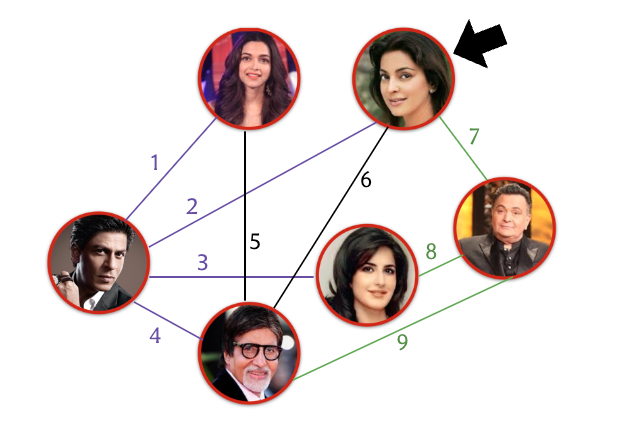
\includegraphics{./figures/ch3-eulerpath.png}
}

\caption{An actor collaboration graph}

\end{figure}

This activity is an adaptation of the example from the
\href{https://www.udacity.com/course/intro-to-algorithms--cs215}{Intro
to Algorithms} course at Udacity, where it appears in the first chapter
with the title ``A Social Network Magic Trick''.
\end{tcolorbox}

The question was addressed and answered by Euler (1736). He did not
solve this by ``messing around'' with all possible ways of walking
around the city and checking if any of the walks satisfied the desired
criteria. His more systematic approach involved modeling the problem
abstractly, and making some key observations that ultimately led to the
solution --- not just for this problem, but for all problems with a
similar framing!

Here's another similar-sounding and classic problem involving a
chessboard,
\href{https://en.chessbase.com/post/euler-and-the-knights-tour}{also
posed to Euler}:

\begin{quote}
``I found myself one day in a company where, on the occasion of a game
of chess, someone proposed this question: \emph{To move with a knight
through all the squares of a chess board, without ever moving two times
to the same square, and beginning with a given square.}''
\end{quote}

The origins of this problem --- the so-called ``Knight's Tour'' --- goes
all the way back to the 9th century AD, where it is described in
\href{https://www.ias.ac.in/article/fulltext/reso/025/08/1095-1116}{Rudraṭa's
Kavyalankara}. Here's an example of a knight's tour, as seen on
Wikipedia:

\begin{figure}

{\centering \includegraphics{./figures/ch3-kt-anim.gif}

}

\caption{An animated example of a knight's tour.}

\end{figure}

Although deceptively similar to the problem of the bridges, this is a
different problem with two important contrasts:

\begin{enumerate}
\def\labelenumi{\arabic{enumi}.}
\tightlist
\item
  we were previously not allowed to reuse \emph{bridges}, here we are
  not allowed to reuse \emph{squares}, and
\item
  we were previously obliged to use \emph{every} bridge, here we are
  \emph{not} required to make every possible move that exists.
\end{enumerate}

Generalizing from the 8x8 chessboard, you could ask yourself what
\((n \times n)\) boards admit such tours.

\begin{tcolorbox}[standard jigsaw,toptitle=1mm, titlerule=0mm, bottomtitle=1mm, title=\textcolor{quarto-callout-warning-color}{\faExclamationTriangle}\hspace{0.5em}{(Spoiler) Numberphile commentary on the knight's tour}, coltitle=black, colback=white, toprule=.15mm, colframe=quarto-callout-warning-color-frame, arc=.35mm, rightrule=.15mm, opacityback=0, left=2mm, leftrule=.75mm, colbacktitle=quarto-callout-warning-color!10!white, opacitybacktitle=0.6, bottomrule=.15mm]

\end{tcolorbox}

\hypertarget{abstractions-via-graphs}{%
\section{Abstractions via Graphs}\label{abstractions-via-graphs}}

It's useful to model such problems using \emph{graphs} (aka
\emph{networks}). And we're not talking sine curves here --- a graph in
our context is a structure that represents relationships between
entities.

Usually these relationships are between two entities at a time. Indeed,
this is typically already quite a bit to keep track of, hence graphs
that do more are said to be hyper. That is to say, graphs that model
relationships involving more than two entities in one go are generally
called \emph{hypergraphs}, and they will be a story for another day.

For now, we will variously refer to entities as \emph{vertices} or
\emph{nodes}, and relationships as \emph{edges} or \emph{connections}.
Come to think of it, graphs are everywhere:

\begin{longtable}[]{@{}
  >{\raggedright\arraybackslash}p{(\columnwidth - 2\tabcolsep) * \real{0.3140}}
  >{\raggedright\arraybackslash}p{(\columnwidth - 2\tabcolsep) * \real{0.6860}}@{}}
\toprule()
\begin{minipage}[b]{\linewidth}\raggedright
Entities
\end{minipage} & \begin{minipage}[b]{\linewidth}\raggedright
Two entitites are in a relationship if\ldots{}
\end{minipage} \\
\midrule()
\endhead
People & they are in a relationship. \\
Cats & they have fought each other. \\
Actors & they have been in a movie together. \\
Airports & there is a direct flight between them. \\
Landmasses & there is a bridge connecting them. \\
Songs & one of the tunes was copied from the other. \\
Subsets of \([42]\) & one is contained in another. \\
Ingredients & there is a recipe that uses them together. \\
Webpages & one of them has a link leading to the other. \\
Twitter Users & one of them follows the other\footnote{Find out more
  about \href{https://dl.acm.org/doi/10.1145/2488388.2488433}{Twitter's
  WTF (who-to-follow) service}.} \\
Locations on a Chessboard\footnote{See how the puzzle about exchanging
  the positions of black and white knights can be
  \href{https://www.nytimes.com/2022/07/05/science/june-huh-heisuke-hironaka-math-chromatic-geometry.html}{recast
  as a graph problem}.} & one of them is reachable from the other via a
knight move. \\
\bottomrule()
\end{longtable}

We usually like to distinguish between graphs where the relationships
are potentially one-sided (such as people in a relationship), and those
where they are mutual (such as ingredients in a recipe). Edges like
these are called \emph{directed} and \emph{undirected}, respectively.

Depending on what the graph is modeling, we may not allow for entities
to entertain relationships with themselves (e.g, flights don't come back
to airports they took off from). In other contexts, it makes sense to
allow for this (e.g, a set always contains itself). An edge that
connects a vertex to itself is called a \emph{self-loop}\footnote{There
  are even graphs that
  \href{https://en.wikipedia.org/wiki/Bouquet_graph}{\emph{only} have
  self-loops}.}.

Sometimes, it is reasonable that there are multiple edges between a
fixed pair of vertices (for example, consider that there are several
recipies that use salt and potatoes). Multiple edges are useful to model
a multitude of relationships, and are often called \emph{multiedges}
when used.

A \emph{simple} graph is one that does not have either self-loops or
multiedges.

Finally, it is worth mentioning that some relationships naturally
connect more two entities. For example, in an actor collaboration graph,
you would find edges between Amitabh Bachchan, Juhi Chawla, and Shah
Rukh Khan. You would also find edges between Akshay Kumar, Dhanush, and
Sonam Kapoor. In the first example, there happens to be one film that
all three actors feature in together, while this is not the case in the
latter, at least at the time of this writing. As such, the graph does
not have enough structure to reveal this distinction: it looks exactly
the same in both cases!

For an actor-collaboration graph, allowing for \(n\)-way relationships
would make room for accurately capturing information about both actors
and movies. Indeed, every movie could be represented by an `edge' ---
the subset of actors who belonged to the cast. Such graphs are called
\emph{hypergraphs} or \emph{set systems}.

While hypergraphs are a very useful generalization of graphs, they will
be largely out of scope for our discussions in this course. To make up
for that, here is a different workaround to capture all the information
we have in the actor-collaboration graph example. Instead of having a
vertex for every actor, we introduce a vertex for every actor \emph{and}
for every movie. Now, an actor \(a\) and a movie \(m\) are connected by
an edge if \(a\) belongs to the cast of \(m\). Observe that this
approach can be used to ``convert'' any hypergraph into a graph.

A little more terminology before we move on: I promise that we're almost
done introducing new words!

For an undirected graph, a vertex \(u\) is called a \emph{neighbor} of a
vertex \(v\) if \((u,v)\) is an edge. For a directed graph, the presence
of the edge \((u,v)\) would make \(v\) an \emph{out-neighbor} of \(u\)
and \(u\) an \emph{in-neighbor} of \(v\).

For an undirected graph, the \emph{degree} of a vertex \(v\) is the
number of neighbors of \(v\). For a directed graph, the in-degree and
out-degree of \(v\) is the number of in-neighbors and out-neighbors of
\(v\), respectively.

\hypertarget{representing-graphs}{%
\section{Representing Graphs}\label{representing-graphs}}

If you wanted to tell your program about a graph, there are a few
different ways you could go about it. Let's assume that we're trying to
represent a graph \(G\) on \(n\) nodes, labeled \(1\) through \(n\), and
\(m\) edges.

\begin{tcolorbox}[standard jigsaw,toptitle=1mm, titlerule=0mm, bottomtitle=1mm, title=\textcolor{quarto-callout-caution-color}{\faFire}\hspace{0.5em}{How would you do it?}, coltitle=black, colback=white, toprule=.15mm, colframe=quarto-callout-caution-color-frame, arc=.35mm, rightrule=.15mm, opacityback=0, left=2mm, leftrule=.75mm, colbacktitle=quarto-callout-caution-color!10!white, opacitybacktitle=0.6, bottomrule=.15mm]

Before reading further, it would be worth spending some time thinking
about how you would represent a graph. Based on our discussions so far,
you might counter this with the question: ``Well, what do \emph{you}
need it for?'' --- and that's a fair reaction!

Listed below are some fairly common operations that come up when dealing
with graphs.

\begin{Shaded}
\begin{Highlighting}[]
\NormalTok{1. add edge u v}
\NormalTok{2. remove edge u v}
\NormalTok{3. add vertex v}
\NormalTok{4. remove vertex v}
\NormalTok{5. find degree v}
\NormalTok{6. find maxdegree G}
\NormalTok{7. find mindegree G}
\end{Highlighting}
\end{Shaded}

\end{tcolorbox}

\textbf{Edge Lists.} The most natural way is to perhaps just braindump
the full list of edges. This gives us all we need to know about \(G\).

Since this is just a plain list, you could implement it either as an
array or as a linked list.

\textbf{Adjacency Matrix.} The other way is to block off a
\(n \times n\) array \(A\) of integers. You could then have:

\[ \begin{equation*}
   A[i][j] =
    \begin{cases}
      1 & \text{if } (i,j) \in E,\\
      0 & \text{otherwise.}
    \end{cases}
\end{equation*}
\]

\textbf{Adjacency Lists.} Finally, you could have an array \(A\) of size
\(n\), with \(A[i]\) pointing to a list of the neighbors of the vertex
\(i\) if the graph is undirected, and out-neighbors if the graph is
directed.

Again, since these are just lists, they could be, in principle,
implemented either as arrays or linked lists. We will follow the
traditional choice of implementing them as lists.

It should be no surprise at this point that there is no ``right'' answer
to the choice of representation. You might have noticed, for instance,
that an adjacency matrix always reserves \(n^2\) units of space to store
\(G\), while the amount of space consumed by the other two
representations is proportional to \(m\). Notice that the number of
edges in a graph can be as large as \(\approx n^2\) for simple graphs,
so there certainly are graphs for which the space consumption looks the
same for all representations. However, for graphs where there aren't as
many edges, then the matrix representation is likely wasteful in terms
of space, although you may have other good reasons for sticking to it.

Let's classify expenses incurred as follows.

\begin{enumerate}
\def\labelenumi{\arabic{enumi}.}
\tightlist
\item
  \textbf{Brilliant.} When the procedure only needs constant time.
\item
  \textbf{Decent.} When the procedure always wraps up in, and sometimes
  needs, time proportional to the maximum degree of the graph.
\item
  \textbf{(n/m)-tolerable.} When the procedure always wraps up in, and
  sometimes needs, time proportional to the number of vertices/edges in
  the graph.
\item
  \textbf{(n/m)-painful.} When the procedure always wraps up in, and
  sometimes needs, time proportional to the number of vertices/edges in
  the graph squared.
\end{enumerate}

Here's a run down of how the representations above fare with respect to
some of the common operations mentioned in the opening exercise.

\begin{longtable}[]{@{}cccc@{}}
\toprule()
Operations & Adj. Matrix & Adj. List & Edge List \\
\midrule()
\endhead
Adding a vertex & n-Painful & n-Tolerable & Decent \\
Deleting a vertex & n-Painful & n-Tolerable & m-Tolerable \\
Adding an edge & Brilliant & Brilliant & Brilliant \\
Deleting an edge & Brilliant & Decent & m-Tolerable \\
Finding degree(v) & n-Tolerable & Decent & m-Tolerable \\
Check if (u,v) is an edge & Brilliant & Decent & m-Tolerable \\
\bottomrule()
\end{longtable}

It would be a good exercise to validate that these claims indeed make
sense.

Now that we're comfortable with storing graphs, next up, we'll talk
about exploring them.



\end{document}
